
\documentclass[10pt,a4paper]{article}

% ─── Packages ─────────────────────────────────────────
\usepackage{fontspec}
\setmainfont{Times New Roman}

\usepackage[top=1.1cm,bottom=1.1cm,left=1.55cm,right=1.55cm]{geometry}
\usepackage{titlesec}
\usepackage{enumitem}
\usepackage{hyperref}
\usepackage{xcolor}
\usepackage{tabularx}
\usepackage{graphicx}
\usepackage{parskip}

% ─── Colors ───────────────────────────────────────────
\definecolor{primary}{RGB}{30,40,90}
\definecolor{namecolor}{RGB}{0,120,180}
\definecolor{accent}{RGB}{50,90,150}
\definecolor{rulecol}{RGB}{200,205,220}
\definecolor{gray}{RGB}{90,90,90}

\hypersetup{
    colorlinks=true,
    urlcolor=accent
}

\pagestyle{empty}
\setlength{\parskip}{0pt}

% ─── Section ──────────────────────────────────────────
\titleformat{\section}
    {\normalsize\bfseries\color{primary}}
    {}
    {0em}
    {}
    [\vspace{1pt}\textcolor{rulecol}{\titlerule[0.6pt]}\vspace{1pt}]

\titlespacing{\section}{0pt}{5pt}{2pt}

% ─── Entry ────────────────────────────────────────────
\newcommand{\entry}[3]{%
    \noindent
    \begin{tabularx}{\linewidth}{X r}
        \textbf{\color{primary}#1} &
        {\scriptsize\color{gray}#2}
    \end{tabularx}\\[-2pt]
    {\scriptsize\textit{\color{gray}#3}}
    \vspace{1pt}
}

% ─── Compact list ─────────────────────────────────────
\newenvironment{cvitems}{
    \begin{itemize}[
        leftmargin=1.15em,
        topsep=0pt,
        itemsep=0.5pt,
        parsep=0pt,
        partopsep=0pt
    ]
}{
    \end{itemize}
}

% ═════════════════════════════════════════════════════
\begin{document}

% ─── HEADER ───────────────────────────────────────────
\noindent
\begin{tabularx}{\linewidth}{@{}X r@{}}

\begin{minipage}[c]{\linewidth}

    {\LARGE\bfseries\color{namecolor} Ho Huynh Nhu}\\[2pt]

    {\large\bfseries\color{primary}
    Data Scientist}\\[3pt]

    {\scriptsize\color{gray}
    20/10/2003
    \enspace\textcolor{rulecol}{|}
    \enspace (+84) 367 503 477
    \enspace\textcolor{rulecol}{|}
    \enspace
    \href{mailto:hhnhu2003@gmail.com}{hhnhu2003@gmail.com}
    \enspace\textcolor{rulecol}{|}
    \enspace Ho Chi Minh City}\\[2pt]

    {\scriptsize
    \href{https://github.com/hohuynhnhu}
    {github.com/hohuynhnhu}
    \enspace\textcolor{rulecol}{|}
    \enspace
    \href{https://www.facebook.com/huynhnhu.ho.961}
    {facebook.com/huynhnhu.ho.961}
    }

\end{minipage}

&

\begin{minipage}[c]{2.2cm}
    \raggedleft
    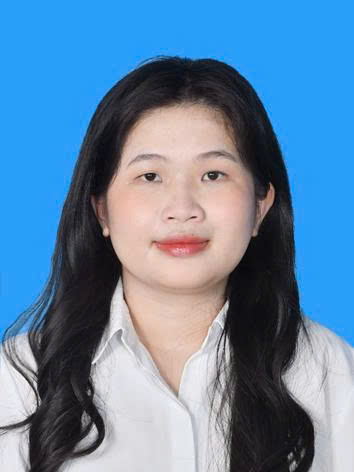
\includegraphics[
        width=2.2cm,
        height=2.7cm,
        keepaspectratio
    ]{assets/avt.jpg}
\end{minipage}

\end{tabularx}

\vspace{3pt}
\textcolor{rulecol}{\rule{\linewidth}{0.6pt}}

% ─── CAREER OBJECTIVE ─────────────────────────────────
\section*{Career Objective}

{\small
Final-year Information Technology student pursuing a Data Scientist
career, with hands-on experience in Python, SQL, data processing,
machine learning, and data pipelines. Experienced in data preparation,
exploratory analysis, feature engineering, model training, evaluation,
and data visualization. Seeking a Data Scientist position to apply
data-driven approaches to real-world business problems.
}

% ─── EDUCATION ────────────────────────────────────────
\section*{Education}

\entry
{University of Transport Ho Chi Minh City (UTH)}
{10/2022 -- 10/2026}
{Bachelor of Information Technology -- Completed coursework}

{\small
\begin{cvitems}
    \item GPA: 3.4 / 4.0
    \item \textbf{Excellent Scholarship} -- Semester 1, 2025
    \item \textbf{Second Prize -- AI Track},
    UTH Student Scientific Research Conference 2025
\end{cvitems}
}

% ─── TECHNICAL SKILLS ─────────────────────────────────
\section*{Technical Skills}

{\small
\begin{tabularx}{\linewidth}{@{}lX@{}}

\textbf{Data Science}
&
Python, Pandas, NumPy, Scikit-learn, EDA,
Data Cleaning, Feature Engineering, Statistical Analysis
\\[1pt]

\textbf{Machine Learning}
&
Supervised Learning, Classification, Regression,
Decision Tree, Random Forest, Model Evaluation, Cross-Validation
\\[1pt]

\textbf{Deep Learning}
&
PyTorch, CNN, Siamese Network, Transformer,
YOLO, MediaPipe
\\[1pt]

\textbf{Data Engineering}
&
ETL/ELT, Data Pipeline, dbt, Apache Airflow,
Data Lake, Data Warehouse
\\[1pt]

\textbf{SQL / Database}
&
SQL, PostgreSQL, SQL Server, MongoDB,
Firebase, Supabase
\\[1pt]

\textbf{Data Visualization}
&
Power BI, Metabase, DAX, Matplotlib, Seaborn
\\[1pt]

\textbf{Programming}
&
Python, SQL, TypeScript, JavaScript, Kotlin
\\[1pt]

\textbf{Tools}
&
Git, Docker, Postman, VS Code

\end{tabularx}
}

% ─── WORK EXPERIENCE ──────────────────────────────────
\section*{Work Experience}

\entry
{Gotik Consulting -- Data Engineer}
{Python \textbar{} dbt \textbar{} PostgreSQL \textbar{} Airflow}
{03/2026 -- 05/2026}

{\small
\begin{cvitems}

    \item Processed and transformed Odoo data to prepare structured
    datasets for analytics and reporting.

    \item Developed Python data pipelines and dbt data models using
    PostgreSQL, and automated hourly ETL workflows with Airflow.

    \item Prepared analytical datasets and developed Power BI dashboards
    for operational monitoring and data-driven insights.

\end{cvitems}
}

% ─── PROJECTS ─────────────────────────────────────────
\section*{Featured Data Science Projects}

\entry
{Fall Detection -- Machine Learning Classification System}
{Python \textbar{} PyTorch \textbar{} YOLOv8 Pose \textbar{} MediaPipe \textbar{} Transformer}
{04/2026 -- 06/2026}

{\small
\begin{cvitems}

    \item Prepared video datasets and extracted human pose features
    using MediaPipe and YOLOv8 Pose for fall/non-fall classification.

    \item Developed and trained a Transformer Encoder for binary
    classification using sequential pose features.

    \item Achieved 97.8\% mean accuracy with 5-fold cross-validation
    and evaluated model performance on unseen data.

\end{cvitems}
}

\vspace{3pt}

\entry
{VehicleScan -- AI-Based Vehicle Recognition System}
{Python \textbar{} YOLO \textbar{} CNN \textbar{} Siamese Network \textbar{} Firebase}
{03/2025 -- 03/2026}

{\small
\begin{cvitems}

    \item Prepared and labeled datasets for vehicle detection,
    classification, and recognition tasks.

    \item Trained and evaluated YOLO, CNN, and Siamese Network models
    for vehicle identification and recognition.

    \item Applied image preprocessing and feature extraction, and
    achieved Second Prize -- AI Track at UTH 2025.

\end{cvitems}
}

% ─── ADDITIONAL INFORMATION ───────────────────────────
\section*{Additional Information}

{\small
\begin{tabularx}{\linewidth}{@{}lX@{}}

\textbf{Soft Skills}
&
Problem-solving \textbar{}
Analytical thinking \textbar{}
Research and self-learning \textbar{}
Teamwork \textbar{}
Troubleshooting
\\[2pt]

\textbf{Data Science Interests}
&
Data Analysis \textbar{}
Machine Learning \textbar{}
Predictive Modeling \textbar{}
Deep Learning \textbar{}
Data Visualization
\\[2pt]

\textbf{Other}
&
Experience working with data pipelines, databases,
data warehouses, machine learning models, and BI dashboards.
\\[2pt]

\textbf{Availability}
&
Available for full-time Data Scientist / Junior Data Scientist
opportunities and willing to adapt to job requirements.

\end{tabularx}
}

\end{document}

